%%%%%%%%%%%%%%%%%%%%%%%%%%%%%%%%%%%%%%%%%%%%%%%%%%%%%%%%%%%%%%%%%%%
%
% This is a general template file for the LaTeX package SVJour3
% for Springer journals.          Springer Heidelberg 2010/09/16
%
% Copy it to a new file with a new name and use it as the basis
% for your article. Delete % signs as needed.
%
% This template includes a few options for different layouts and
% content for various journals. Please consult a previous issue of
% your journal as needed.
%
%%%%%%%%%%%%%%%%%%%%%%%%%%%%%%%%%%%%%%%%%%%%%%%%%%%%%%%%%%%%%%%%%%%
%
\RequirePackage{fix-cm}
%
\documentclass[twocolumn]{svjour3}
%
\smartqed
%
\usepackage{graphicx}
\usepackage{hyperref}
\usepackage[round, sort&compress, numbers]{natbib}
\usepackage{multirow}
\usepackage{graphicx}
\usepackage{units}
\usepackage{color}
\usepackage{xspace}
%
\DeclareRobustCommand\IPCClongname{}
%
% please place your own definitions here and don't use \def but \newcommand{}{}
\newcommand{\pmlib}{\texttt{pmlib}\xspace}
%
% Insert the name of "your journal" with
% \journalname{myjournal}
%
\begin{document}

\title{Evaluating the Performance  and Energy Efficiency of COSMO-ART,
  a Fully Online Coupled  Model System with Numerical Weather Forecast
  and Chemical Transport Models }
% \thanks{This work was supported by the EU Project FP7 318793 ``EXA2GREEN''}}
%\subtitle{Write here subtitle}

%\titlerunning{Short form of title} % if too long for running head

\author{Joseph~Charles  \and William~Sawyer  \and  Manuel~F.~Dolz \and
  Cristiano~Malossi}

%\authorrunning{Short form of author list} % if too long for running
%head

\institute{J.~Charles, W.~Sawyer 
	\at Swiss National Supercomputing Centre (CSCS)
	\\ CH-6900 Lugano, Switzerland  
	%\\ Tel: +41  (0) 91  610 8216
 	\\ E-mails:~{\{joseph.charles,william.sawyer\}@cscs.ch} 
        \and M.~F.~Dolz 
        \at Dept. of Informatics, University of Hamburg
	\\ D-22.527 Hamburg, Germany
        %\\ Tel: +49 (0) 40 460094-404
        \\ \email{manuel.dolz@informatik.uni-hamburg.de}  
        \and C.~Malossi  
        \at IBM Zurich Research Laboratory 
        \\  CH-8000 Zurich, Switzerland
        %\\  Tel: +41 (0) 44 724 8616
        \\ \email{ACM@zurich.ibm.com}}

\date{Received: date / Accepted: date} % The correct dates will be
                                       % entered by the editor

\maketitle

\begin{abstract}
  In this paper we present  COSMO-ART, an extension of the operational
  weather  forecast  model  of   the  German  weather  service  (DWD),
  developed for  the evaluation of the interactions  of reactive gases
  and aerosol particles  with the state of atmosphere  at the regional
  scale. It  includes secondary aerosols,  directly emitted components
  like  soot,  mineral  dust,  sea  salt and  biological  material  as
  pollen. Processes such  as emissions, coagulation, condensation, dry
  deposition,  wet removal,  and sedimentation  of aerosols  are taken
  into account.   The overall performance  of this application  on HPC
  systems is analysed  by a profiling study to  determine hotspots and
  identify critical paths.   Moreover, we describe measurement devices
  and  energy-aware   techniques  employed  to   evaluate  the  energy
  footprint of the considered application and to get detailed insights
  about power bottlenecks.  Our motivation is to improve corresponding
  code   sections  to  sustain   high  performance   while  minimizing
  energy-to-solution.   This  preliminary  work  sets  the  basis  for
  subsequent studies to tackle  challenges related to energy efficient
  high performance computing in the framework of the Exa2Green project
  (\url{http://exa2green.eu/}).

\keywords{High performance computing  \and Energy-aware computing \and
  Green computing  \and Numerical weather  prediction \and Atmospheric
  chemistry  \and  Aerosols  modelling  \and  Profiling  methods  \and
  Benchmark analysis \and COSMO-ART coupled model}
% \PACS{PACS code1 \and PACS code2 \and more}
% \subclass{MSC code1 \and MSC code2 \and more}
\end{abstract}

\section{Introduction}
\label{intro}
While anthropogenic greenhouse gas emissions are driving unprecedented
major  climate  changes  since   the  mid-20$^{th}$  Century,  one  factor
overwhelmingly  affects  the  uncertainty  in  determining  human-induced
radiative  forcing:  the  effects   of  aerosols  in  the  atmosphere.
Although they  are not considered  heat-trapping greenhouse  gases and
have  shorter  atmospheric lifetimes,  aerosols  significantly modify  the
global   radiation   budget   \citep{IPCC-2013}.   Enhanced   aerosols
concentrations impact the climate  system by scattering and absorption
of solar radiation, thereby exerting a direct radiative forcing; or by
modifying cloud  properties,  cloud  fraction and  surface
albedo,  causing  a  negative  indirect  radiative  forcing.   Despite
considerable  progress in  global aerosol  modelling \citep{Mann-2013}
and  measurement-based  assessments,  large  uncertainties  remain  in
current  estimates  of  aerosol radiative  forcing  \citep{Myhre-2013,
IPCC-2013,  Lee-2013,   Randles-2013,  Rosenfeld-2013,  Sherwood-2013,
Stier-2013}.

Hence to  improve our understanding of  aerosol-cloud interactions and
reduce  these  uncertainties,  the  research  community  is  making  a
concerted international  effort to represent  the underlying physical,
chemical  and aerosol dynamical  processes through  numerical chemical
transport  models (CTMs)  such  as ART  (Aerosols  and Reactive  Trace
gases),   developed   at  the   Karlsruhe   Institute  of   Technology
(KIT)  \citep{Vogel-2009,  Bangert-2011,  Knote-2013}.  This  regional
scale modelling system is coupled  with the operational  weather forecast
model  \textsc{Cosmo}  \citep{Baldauf-2011},  jointly developed and used by  a
consortium of European weather centers, as well as utilised in a climate version
by the wider research community.

The extended  atmospheric model \textsc{Cosmo-art}  is com\-put\-ationally
much  more  demanding than  \textsc{Cosmo}  since  a  large number  of
additional  tracers and  processes have  to be  considered.   Thus the
model  is currently  severely limited  in terms  of applicability  and
expensive in terms of energy consumption.  Although \textsc{Cosmo} has
recently been ported to GPUs \citep{Gysi-2014, Lapillonne-2014} within
the framework of the  High Performance and High Productivity Computing
(HP2C) Initiative  \citep{HP2C} to optimise it  for computational and
energy efficiency,  significant investments in ART  are still required
to take it  to a similar level.  The  efficiency of \textsc{Cosmo-art}
is being  addressed in the  EU Exa2Green project  \citep{EXA2GREEN} to
deliver a  prototype code, which  provides an energy efficiency  of at
least five times the  baseline value.  Such an implementation would
allow  the  community  to  investigate critical  questions  at  higher
resolution  and   over  longer  periods,   at  reduced  cost   to  the
environment.

This  work is  organized as  follows: in  Sec.~\ref{sec:1} we  give an
overview  of  related  work,   then  in  Sec.~\ref{sec:2}  we  briefly
introduce \textsc{Cosmo-art}  and specify its  technical setup related
to  the investigated  performance and  energy evaluation  methods.  In
Sec.~\ref{sec:3}   we  describe   HPC  platforms,   power  measurement
equipments   and  software  environment   employed  to   conduct  this
benchmarking study.  Sec.~\ref{sec:4}  presents performance and energy
requirements  of the  baseline on  these architectures  and highlights
areas where improvements will be necessary for the subsequent baseline
refactoring.   Finally,  we  conclude in Sec.~\ref{concl} with some 
implications for the Exa2Green project and give an outlook for future
research.


\section{The COSMO-ART model system}
\label{sec:1}
\subsection{Model description}
\label{subsec:1.1}
COSMO-ART  (ART  stands  for   Aerosols  and  Reactive  Trace  gases),
developed  at  KIT  Karlsruhe  \citep{Vogel-2009}, is  a  regional  to
continental scale model coupled  online to the COSMO numerical weather
prediction  (NWP) and  climate  model \citep{Baldauf-2011}.   Physical
processes  like  transport,  turbulent  diffusion,  and  dry  and  wet
deposition  are  treated  together  with  photochemistry  and  aerosol
dynamics using  the modal  approach.  Aerosols dynamics  are simulated
with the modal aerosol module MADE \citep{Ackermann-1998}, improved by
explicit  treatment of  soot aging  through condensation  of inorganic
\citep{Riemer-2003}   and   organic   substances   (MADEsoot),   which
represents the  aerosol population using  eleven overlapping lognormal
modes.   Five  modes  represent  sub-micron  particles  consisting  of
sulphate,  ammonium,  nitrate,   organic  compounds,  water  and  soot
\citep{Riemer-2004}  in a  range  of mixing  state.   These modes  are
coupled with  the gas  phase by condensation  and nucleation,  and are
strongly influenced by anthropogenic emissions of gases and particles.
Sea    salt     \citep{Lundgren-2013},    mineral    dust    particles
\citep{Vogel-2006, Stanelle-2010}  and rest anthropogenic  species are
treated by  seven additional modes. For each  mode, mass contributions
and total  number concentration  are prognostic quantities,  while the
standard deviation is fixed.

Specific  modules are included  to simulate  the dispersion  of pollen
grains    \citep{Vogel-2008}   and    other    biological   particles.
Meteorologically-influenced emissions  are also online  coupled within
the  model  system.  The  biogenic  VOC  (volatile organic  compounds)
emissions are  calculated as functions of  the land use  type based on
the Global  Land Cover 2000  dataset and the modeled  temperatures and
radiative fluxes \citep{Vogel-1995}.

The gaseous chemistry in COSMO-ART  is solved by a modified version of
the  Regional  Acid  Deposition  Model, Version  2  (RADM2)  mechanism
\citep{Stockwell-1990},  which  is   extended  to  describe  secondary
organic aerosol formation based on a volatile basis set (VBS) approach
\citep{Athanasopoulou-2013}  and  hydroxyl  radical recycling  due  to
isoprene chemistry \citep{Geiger-2003}.  The thermodynamic equilibrium
between the  gas and particulate  phases of the inorganic  material is
achieved through the  ISORROPIA II module \citep{Fountoukis-2007}. 

COSMO-ART  is  fully  online-coupled,  and  allows  for  feedbacks  of
aerosols  on  temperature,  radiation  and cloud  condensation  nuclei
(CCN).   Analytical  description  of  modules  incorporated  for  this
purpose  exists in  \citep{Vogel-2009,  Bangert-2011}.  The  radiation
scheme used  within the  model to calculate  the vertical  profiles of
shortwave and longwave radiative fluxes is GRAALS \citep{Ritter-1992}.
In order to account for  the interaction of aerosol particles with the
cloud microphysics and radiation,  COSMO-ART uses the two-moment cloud
microphysics  scheme of  Seifert and  Beheng  \citep{Seifert-2006} and
comprehensive parameterizations for cloud condensation and ice crystal
nucleation  \citep{Bangert-2011, Bangert-2012}.   The system  of stiff
ordinary differential equations described by chemical reactions in the
aqueous-phase together with the transfer reactions is solved using the
Kinetic PreProcessor (KPP, \citealp{Damian-2002}).

Detailed  model  description  can   be  found  in  the  aforementioned
publications  as   well  as  in   \citep{Stanelle-2010,  Bangert-2012,
  Knote-2011, Knote-2013}.

\subsection{Model setup}
\label{subsec:1.2}
To define a baseline within a code under development, it was necessary
to  find  a  run-configuration  capable  of  being  recreated  in  all
subsequent versions. The  energy-to-solution benchmarking of COSMO-ART
concerns  one-day  long simulations  without  spin-up  stage, using  a
222x216x40  discretization of  Europe and  a  time step  of 120s.  The
baseline code incorporates 34 2-d and  45 3-d fields to be written out
every hour for a simulation starting  on April 13th, which is close to
the equinox and thus brings  benefits of having approximately half day
of night and  half day of sun exposure, to  ensure a proper activation
of  the chemistry  cycle. Ultimately  new  input files  closer to  the
equinox (on March 20th) will be  created, but the current set of input
files is fine for the time being.

This COSMO-ART  version is configured  to deal with a  semi Lagrangian
horizontal advection scheme  with tricubic interpolation and selective
filling diffusion option in combination with the Runge-Kutta dynamical
core.   Concerning the modelling  of wet  deposition in  aerosols, the
baseline  has  only  indirect  cloud  feedbacks  but  doesn't  include
in-cloud  scavenging (rainout)  and  below-cloud scavenging  (washout)
yet.  Amongst  physical parameterizations, precipitation  formation is
performed  by a  two-moment  cloud microphysics  scheme  instead of  a
classical  bulk microphysics  scheme. Another  important point  is the
fact that  this version makes  use of the Kinetic  PreProcessor solver
for  the  resolution of  atmospheric  chemistry ordinary  differential
equations.


\section{Power-performance measurement framework}
\label{sec:2}
\subsection{Hardware description}
\label{subsec:2.1}
While hardware  platforms mature  and are replaced,  we have  chosen a
state-of-the-art  Intel's third-generation  Core (aka  ``Ivy Bridge'')
processing platform (called ``Monch'')  for our power measurements, as
it  is slated  to stay  in service  without hardware  upgrade  for the
duration  of  the Exa2Green  project.   In  principle  at least,  this
architecture could be recreated or found in an identical configuration
beyond the lifetime of the project.  Given that the baseline benchmark
can    be    reproduced    within    an   expected    variance    (see
subsection~\ref{subsec:1.2}), and that  the baseline run configuration
can be used in all future versions of the code, a fair comparison will
be made between the baseline  and the milestone versions of COSMO-ART.
In  this   study,  a  complementary   energy-to-solution  benchmarking
comparison is carried out on  the ``Pilatus'' cluster based on Intel's
previous-generation  ``Sandy  Bridge'' processors,  known  to be  more
power consuming.

\subsubsection{Monch (CSCS - ETH Zurich)}
Monch, which is installed  at the Swiss National Supercomputing Center
(CSCS)  of the ETH  Zurich, is  a 10  rack NEC-provided  (LX-2400) and
dual-socket Intel-based cluster, utilised from people that are part of
the   Swiss  Platform   for  Advanced   Scientific   Computing  (PASC,
\url{http://www.pasc-ch.org/}).   It  is   composed  of  312  standard
compute  nodes,  24  large-memory  compute nodes  and  24  huge-memory
compute nodes.   Each standard compute node comprises  2 Intel 10-core
Ivy Bridge EP E5-2660v2 processors operating at 2.2 GHz, offering 32GB
of DDR3 1600MHz  RAM, themselves connected by a  high speed Infiniband
network,  based on Mellanox  SX6036 managed  FDR (Fourteen  Data Rate)
switches, with a 56 Gb/s speed.

\subsubsection{Pilatus (CSCS - ETH Zurich)}
Pilatus is a dual-socket Intel  Sandy-Bridge based cluster used as Piz
Daint pre-post processing cluster.  It is composed of 42 compute nodes
with  a total  number of  1344 cores  in hyper-threading  and  2688 GB
aggregate memory and has 2  high-speed interconnects based on FDR: the
first is  dedicated to the MPI  traffic and the second  to the storage
high  speed traffic.  The  2 login  nodes  and the  42 computes  nodes
consists in  11 twin-pair Intel  E5-Series DALCO r2264i4t  2U scalable
compute  modules.  Each  module contains  4 compute  nodes based  on 2
Intel  8-core Intel  Xeon  E5-2670 processors  operating  at 2.6  GHz,
offering  64GB of  DDR3 1600MHz  RAM, themselves  connected by  a high
speed  Infiniband  network,  based  on  Mellanox  SX6036  managed  FDR
(Fourteen Data Rate) switches, with a 56 Gb/s speed.

\subsection{Power-Performance measurement framework}
\label{subsec:2.2}

\subsubsection{CSCS - ETH Zurich}
E3METER  Intelligent Power Strips  (IPS) and  Monitors (IPM)  are high
quality electricity meters which enable to monitor and optimize energy
consumption of datacenters or large facilities.  A central data logger
- the  E3METER Data Concentrator  - aggregates  all measured  data and
makes them available in various forms (SNMP, Web, etc). Data transfers
between E3METER  IPS and E3METER Concentrator  use reliable narrowband
powerline  communication (PLC)  technology which  avoids the  need for
extra cabling.  It has  one internal temperature sensor. Two dedicated
extension  ports  can be  used  to  measure  external temperature  and
humidity  through E3METER  remote sensors.  It  features non-intrusive
voltage, current and frequency measurement through current transformer
with an accuracy of 1\%.

\subsubsection{University of Hamburg}
To assess the  performance and the energy efficiency  of COSMO-ART, we
employ   a    version   of   the    integrated   framework   presented
in~\cite{energy13}  that  works in  combination  with VampirTrace  and
Vampir,   which  are   profiling/tracing   and  visualization   tools,
respectively.
%The left part of the \vref{fig:Lustre} offers a graphical representation of
%the Lustre architecture; the right depicts the tracing and profiling framework.
To  use our  approach,  COSMO-ART is  compiled  using the  VampirTrace
compiler wrappers, which automatically  instrument the Fortran code of
the  model. Next,  COSMO-ART is  run  on the  nodes, thus  dissipating
certain  amount of  power.  The  server nodes  are connected  to power
measurement  devices that  account for  the  dissipated power/consumed
energy and  send the power data  to the tracing  server.  The attached
VampirTrace \pmlib plugin employs the client API that sends start/stop
primitives in order to gather captured data by the wattmeters onto the
tracing server,  where an  instance of the  \pmlib server  is running.
Once COSMO-ART run is finished, the VampirTrace \pmlib plugin receives
the  power   data  from  the  tracing   server.   The  instrumentation
post-processing generates  the performance trace files  and the \pmlib
plugin inserts the power data into them.

In  addition  to the  power  measurements,  we  also account  for  the
resource utilization values  of the nodes: CPU load,  memory usage and
storage device utilization. % and network utilization.  

We  run special  \pmlib  server  instances on  the  server nodes  that
retrieve these  values from the \texttt{proc}  file system (leveraging
the  \texttt{psutil} Python library).   Thus, \pmlib  plugin instances
running  with the  instrumented  application connect  with the  \pmlib
servers.   Finally,   using  the   Vampir   visualization  tool,   the
power-performance traces  can be easily  analyzed through a  series of
plots and statistics.


\section{Evaluation}
\label{sec:3}
\subsection{Sofware environment}
\label{subsec:3.1}
The  software environment  on Monch  is controlled  using  the modules
framework which gives an easy  and flexible mechanism to access to all
of  the  CSCS  provided  compilers,  tools and  applications.   It  is
particularly  useful for  testing code  portability  between different
compilers  or for  changing  between different  versions  of the  same
compiler.  INT2LM  and the COSMO-ART model are  implemented in Fortran
90 for distributed memory parallel computers using the Message Passing
Interface (MPI).  For  our initial benchmarking, we opted  for the GNU
compiler (gcc/4.8.1) with the -O3  compiler flag as it generally gives
a  good  level  of optimization  and  the  code  runs faster  in  this
configuration  than  when  compiled  with  the  intel  compiler,  also
available on  Monch.  Besides, we installed  the MPICH2 implementation
of MPI (mvapich2/1.9) as well  as the commonly used HDF5 (hdf5/1.8.12)
and NetCDF  (netcdf/4.3.1) libraries in favor of  the traditional GRIB
library  for  the  management  of  extremely large  and  complex  data
collections.    Note   that   the  Linux   2.6.32-358.11.1.el6.x86\_64
operating system was used for all the Monch compute nodes.

\subsection{Run configuration}
\label{subsec:3.2}
The COSMO-ART model uses NAMELIST-input to specify runtime parameters
splitted into several groups:

\begin{itemize}
\item LMGRID: specifying the domain and the size of the grid,
\item RUNCTL: parameters for the model run,
\item TUNING: parameters for tuning physics and dynamics,
\item DYNCTL: parameters for the adiabatic model,
\item PHYCTL: parameters for the diabatic model,
\item COSMO\_ART: parameters for gases and aerosols model,
\item DIACTL: parameters for the diagnostic calculations,
\item SATCTL: controlling computation of synthetic satellite images,
\item IOCTL: controlling the I/O environment,
\item GRIBIN: controlling the grib input,
\item GRIBOUT: controlling the grib output,
\end{itemize}

\noindent
To run COSMO-ART the following input data are necessary:
\begin{itemize}
\item  Gas phase:  Anthropogenic emissions  for different  species and
  land use data for biogenic emissions and deposition,
\item Aerosol particles: Anthropogenic emissions,
\item Mineral dust: Soil specific land use data.
\end{itemize}

A snapshot of the code, which includes, at least conceptually, all the
information needed  to reproduce the  energy-to-solution benchmarks of
COSMO-ART, was  produced and run on a  full rack of 52  nodes on Monch
(monchc[029-080]),  which represents a  total of  1040 cores  using 20
tasks per node.  The calculated region was mapped to the participating
processors  using a 2D-partitioning  strategy. The  distribution along
the  x and  y coordinates  is defined  in the  namelist  INPUT\_ORG by
setting:  $nprocx=40$   and  $nprocy=26$,  as  the   total  number  of
processors has to be equal to $nprocx \times nprocy$.  Besides we take
$nprocio=0$.   Hyperthreading  is  not  considered in  this  study  as
previous attempts  of its  use revealed that  it always led  to higher
energy-to-solution.\\

Multiple production runs of COSMO-ART were performed to illustrate the
reproducibility  of   the  baseline,  and   quantify  the  significant
uncertainties in  the power measurement, as dictated  by the available
technology (see subsection~\ref{subsec:2.2}).

\subsection{Power-measurement results}
\label{subsec:3.3}
Measuring  the power  consumption on  one entire  Cray cabinet  is the
easiest way to calculate energy-to-solution for given applications.

\begin{figure*}
  \includegraphics[width=0.4\textwidth]{Figs/NRJ_benchmark_Monch.eps}
  \caption{Isola E1 Rack 2 Total Power and Isola E1 Total Power}
  \label{fig:1}
\end{figure*}

The run  was issued successfully  twice, the start time  and execution
time for both jobs are:
\begin{itemize}
\item start=12:51:03, end=13:20:46 $\Rightarrow$ T = 00:29:43 = 1783 s
\item start=14:28:40, end=14:58:02 $\Rightarrow$ T = 00:29:22 = 1762 s
\end{itemize}

The power  consumption for  both jobs is  calculated by  averaging the
corresponding power  measurements from the Excel  file.  Power results
account for the  Isola E1 Rack 2 Total Power. As  time resolution is 5
minutes  for the  output  results, the  average  power consumption  is
computed   by  considering  6   values  for   each  single   run  (see
Table~\ref{tab:1}).

\begin{table}
  \begin{center}
    \caption{}
    \label{tab:1}
    \begin{tabular}{lll}
      \hline\noalign{\smallskip}
      Time & Measured power (W) & Average power (W)  \\
      \noalign{\smallskip}\hline\noalign{\smallskip}
      12:55:00 & 1.2355833333e+04 & 1.265852278e+04 \\ 
      13:00:00 & 1.2820266667e+04 &  \\
      13:05:00 & 1.2600743333e+04 &  \\ 
      13:10:00 & 1.2811580000e+04 &  \\
      13:15:00 & 1.2609680000e+04 &  \\
      13:20:00 & 1.2753033333e+04 &  \\
      \noalign{\smallskip}\hline\noalign{\smallskip}
      14:30:00 & 1.2019266667e+04 & 1.258640833e+04 \\ 
      14:35:00 & 1.2632253333e+04 &  \\
      14:40:00 & 1.2779040000e+04 &  \\
      14:45:00 & 1.2753180000e+04 &  \\
      14:50:00 & 1.2610476667e+04 &  \\
      14:55:00 & 1.2724233333e+04 &  \\
      \noalign{\smallskip}\hline
    \end{tabular}
  \end{center}
\end{table}

The  total  energy to  solution  is  the straightforward  calculation:\\  

Energy-to-solution  =  Integral  of  power consumption  over  the  job
duration

Often  the  average  power  consumption  times  the  job  duration  is
sufficient.

Thus, the total energy consumption corresponds to: 
\begin{itemize}
\item E  = 1783 x 12658.52278  = 22570146.11674 J $\sim$  22.57 MJ per
  day of simulation
\item E  = 1762 x 12586.40833  = 22177251.47746 J $\sim$  22.18 MJ per
  day of simulation
\end{itemize}


\section{Related work}
\label{sec:4}
\input{Sec4:Related.tex}

\section{Conclusion}
\label{concl}
We  have   presented  a  methodology  for   comparing  performance  of
COSMO-ART,  a  regional  weather  forecast  model  augmented  for  the
interactions of  reactive gases and aerosol  particles.  The resulting
benchmarks illustrate  that the  best time-to-solution does  not imply
the best energy-to-solution: an Intel Sandybridge (2.6 GHz) system has
lower  time-to-solution but  higher energy-to-solution  than  an Intel
Ivybridge  (2.2  GHz) system,  although  the  two  metrics are  indeed
strongly  correlated. On the other hand, the usage of energy-friendly MPI waiting techniques analzyed with our power-performance framework over a series of runs of \cosmoart on \tinto and
power traces demonstrate that it is possible to reduce both
power dissipation and energy-to-solution while maintaining (or even decreasing) the time-to-solution. The  resulting profiles indicate that simple
changes, such as making use of the blocking MPI policy rather
than the polling is possible to slightly reduce both power dissipation and energy consumption (by 2\,\%).

This  reproducible  benchmark provides  a  baseline  for ongoing  work
package within  the EU-funded Exa2Green to  minimise power consumption
of COSMO-ART. Profiling  has given us insight into  the most expensive
code  components,  which are  now  being  altered  to utilise  revised
algorithms.  The  results of these  optimisations will be  reported in
future publications.


%\paragraph{Paragraph headings} Use paragraph headings as needed.

%\begin{figure*}
%  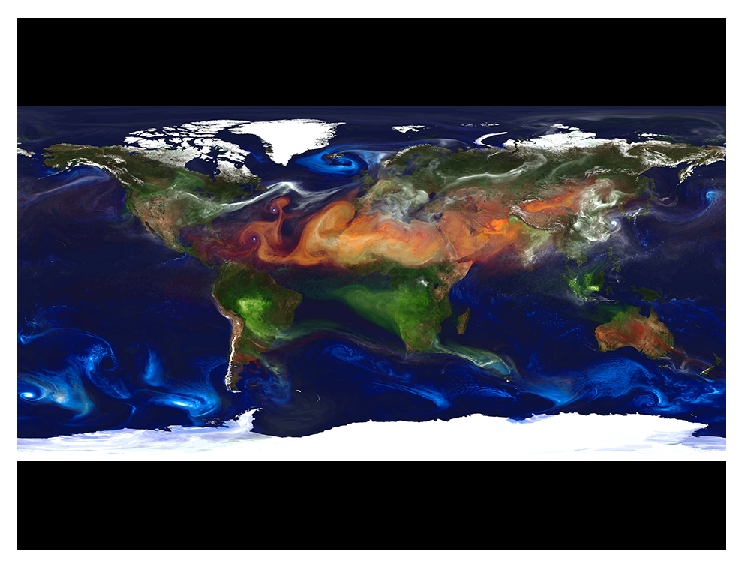
\includegraphics[width=0.4\textwidth]{Figs/earth.eps}
%  \caption{Please write your figure caption here}
%  \label{fig:1}
%\end{figure*}

%\begin{table}
%  \caption{Please write your table caption here}
%  \label{tab:1}
%  \begin{tabular}{lll}
%    \hline\noalign{\smallskip}
%    first & second & third  \\
%    \noalign{\smallskip}\hline\noalign{\smallskip}
%    number & number & number \\
%    number & number & number \\
%    \noalign{\smallskip}\hline
%  \end{tabular}
%\end{table}

\begin{acknowledgements}
This  research  was  supported   by  the  Exa2Green  research  project
co-funded  under the  EU  7th Framework  Program  Future and  Emerging
Technologies (FET) Proactive Initiative: Minimising Energy Consumption
of Computing to  the Limit (MINECC).  The authors  would like to thank
the  High  Performance  and  High  Productivity  Computing  Initiative
(\url{www.hp2c.ch}) for  results that will be  leveraged in subsequent
code refactoring.
\end{acknowledgements}

\DeclareRobustCommand\IPCClongname{ - Intergovernmental Panel on Climate Change}

\bibliographystyle{plainnat}
\bibliography{\jobname}

\end{document}

